\documentclass[11pt,a4paper]{article}

\usepackage[utf8]{inputenc}
\usepackage[T1]{fontenc}
\usepackage{lmodern}
\usepackage[spanish,es-noquoting,es-noshorthands]{babel}
\usepackage[margin=2.3cm]{geometry}
\usepackage{graphicx}
\usepackage{xcolor}
\usepackage{listings}
\usepackage{booktabs}
\usepackage{tabularx}
\usepackage{enumitem}
\usepackage{fancyhdr}
\usepackage[most]{tcolorbox}
\usepackage[hidelinks]{hyperref}

\definecolor{codebg}{HTML}{F6F8FA}
\definecolor{codeframe}{HTML}{D0D7DE}
\definecolor{keyw}{HTML}{0550AE}
\definecolor{strc}{HTML}{0A3069}
\definecolor{comm}{HTML}{6E7781}
\definecolor{okgreen}{HTML}{1A7F37}
\definecolor{badred}{HTML}{CF222E}

\lstdefinelanguage{yaml}{
  keywords={true,false,null},
  morecomment=[l]{\#},
  morestring=[b]', morestring=[b]",
  sensitive=true
}
\lstset{
  basicstyle=\ttfamily\footnotesize,
  backgroundcolor=\color{codebg},
  frame=single, rulecolor=\color{codeframe},
  keywordstyle=\color{keyw}\bfseries,
  stringstyle=\color{strc},
  commentstyle=\color{comm}\itshape,
  breaklines=true, breakatwhitespace=false,
  columns=fullflexible, keepspaces=true,
  showstringspaces=false,
  numbers=left, numberstyle=\tiny\color{comm}, numbersep=6pt,
  xleftmargin=1.6em, framexleftmargin=1.4em,
  literate={á}{{\'a}}1 {é}{{\'e}}1 {í}{{\'i}}1 {ó}{{\'o}}1 {ú}{{\'u}}1
           {ñ}{{\~n}}1 {Á}{{\'A}}1 {É}{{\'E}}1 {Ó}{{\'O}}1 {→}{{$\rightarrow$}}1 {—}{{---}}1
           {≥}{{$\geq$}}1
}
\lstdefinestyle{plain}{numbers=none, xleftmargin=0pt, framexleftmargin=0pt}

\colorlet{notaback}{blue!3!white}\colorlet{notaframe}{blue!45!black}
\colorlet{avisoback}{red!3!white}\colorlet{avisoframe}{red!55!black}
\colorlet{pendback}{orange!8!white}\colorlet{pendframe}{orange!70!black}
\newtcolorbox{nota}[1][]{colback=notaback, colframe=notaframe,
  fonttitle=\bfseries, title={#1}, boxrule=0.6pt, arc=1.5mm}
\newtcolorbox{aviso}[1][]{colback=avisoback, colframe=avisoframe,
  fonttitle=\bfseries, title={#1}, boxrule=0.6pt, arc=1.5mm}
\newtcolorbox{pendiente}[1][]{colback=pendback, colframe=pendframe,
  fonttitle=\bfseries, title={#1}, boxrule=0.6pt, arc=1.5mm}

\newcommand{\code}[1]{\texttt{#1}}
\newcommand{\metrica}{\code{iris\_prediction\_count\_total}}
\newcommand{\repo}{\href{https://github.com/JES0406/mlops-practica-icai}{\code{JES0406/mlops-practica-icai}}}
\newcommand{\run}[1]{\href{https://github.com/JES0406/mlops-practica-icai/actions/runs/#1}{\code{#1}}}
\newcommand{\commit}[1]{\href{https://github.com/JES0406/mlops-practica-icai/commit/#1}{\code{#1}}}

\pagestyle{fancy}
\fancyhf{}
\lhead{\small MLOps --- Observabilidad con Prometheus, Grafana y GMP}
\rhead{\small Javier Escobar Serrano}
\cfoot{\thepage}

\title{\textbf{Observabilidad del modelo Iris con Prometheus,\\Grafana y Google Managed Prometheus}\\[0.4em]
\large Prácticas Unit 7 (Prometheus\_Grafana y Observabilidad de Modelos)}
\author{Javier Escobar Serrano\\
\small Máster en Inteligencia Artificial --- Ingeniería de Modelos 2026-2027}
\date{26 de noviembre de 2026}

\begin{document}
\sloppy
\maketitle
\thispagestyle{empty}

\begin{abstract}
Este informe documenta las dos prácticas de la Unit 7 sobre el repositorio \repo{}.
En la primera se añade al despliegue local con Docker Compose un stack de observabilidad
Prometheus + Grafana, con la fuente de datos y los dashboards provisionados como código.
En la segunda se instrumenta la API Flask del modelo Iris con \code{prometheus-client}
(contador de predicciones por especie), se verifica en local con Prometheus/Grafana y se
lleva a GKE, donde Google Cloud Managed Service for Prometheus (GMP) descubre los pods con
un recurso \code{PodMonitoring}. Por último se analizan los registros en Cloud Logging y se
construye un dashboard de Cloud Monitoring (Top List y Gauge con alineación Delta).
Se detallan las dificultades encontradas y cómo se resolvieron. Todo el trabajo está en la
rama \code{master} (commits \commit{0c0a330}--\commit{eae92ae}).
\end{abstract}

\newpage
\tableofcontents
\newpage

%=====================================================================
\section{Entorno y preparación}
%=====================================================================

\begin{itemize}[nosep]
  \item Proyecto GCP \code{mlops-icai-a2265f} (MLOps ICAI), zona \code{us-central1-a}.
  \item Repositorio \repo{} con el workflow \code{cml.yaml} de prácticas anteriores
        (entrenamiento con DVC/CML + job \code{deploy-to-gke} con Trivy).
  \item Docker 29.8 y Docker Compose v5.5 en WSL2; \code{gcloud}, \code{kubectl} y \code{gh}.
\end{itemize}

\subsection{Clúster GKE con observabilidad desde el principio}
El clúster de la Unit 4 se había borrado al terminar aquella práctica, así que hubo que
recrearlo con el mismo nombre. En lugar de crearlo y luego aplicar los dos
\code{clusters update} del enunciado, se pasaron las opciones en la creación:

\begin{lstlisting}[language=bash,style=plain]
gcloud container clusters create mlops-gke-cluster --zone us-central1-a --num-nodes 2 \
  --enable-managed-prometheus --logging=SYSTEM,WORKLOAD --monitoring=SYSTEM
\end{lstlisting}

La configuración resultante (\code{report/evidence/unit7-cluster-config.yaml}) confirma
\code{loggingConfig: SYSTEM\_COMPONENTS, WORKLOADS} y
\code{managedPrometheusConfig.enabled: true}; en el clúster aparecen los CRD
\code{podmonitorings.monitoring.googleapis.com} y los pods \code{collector} y
\code{gmp-operator} en el namespace \code{gmp-system}. Las APIs \code{monitoring} y
\code{logging} ya estaban habilitadas en el proyecto.

\subsection{Roles de la cuenta de servicio}
La cuenta de servicio que usa GitHub Actions (\code{modelos@...}) solo tenía
\code{artifactregistry.admin} y \code{container.admin}. Se le añadieron los dos roles que
pide el enunciado:

\begin{lstlisting}[language=bash,style=plain]
SA=serviceAccount:modelos@mlops-icai-a2265f.iam.gserviceaccount.com
gcloud projects add-iam-policy-binding mlops-icai-a2265f --member=$SA --role=roles/logging.admin
gcloud projects add-iam-policy-binding mlops-icai-a2265f --member=$SA --role=roles/monitoring.admin
\end{lstlisting}

%=====================================================================
\section{Práctica Prometheus/Grafana: stack local}
%=====================================================================

\subsection{Docker Compose}
Se añaden los servicios \code{prometheus} y \code{grafana} y el volumen
\code{grafana-storage}. Además, \code{mlops-api} pasa a construirse desde el código local
(\code{build: .}) en vez de usar la imagen publicada en Docker Hub, para que el
\code{docker compose up} incluya el endpoint \code{/metrics} de la segunda práctica sin
tener que publicar imágenes.

\begin{lstlisting}[language=yaml]
services:
  mlops-api:
    build: .
    image: mlops-api:latest
    container_name: mlops-api
    ports:
      - "5000:5000"
  # mlops-web sin cambios (jes0406/mlops-web, API_URL=http://mlops-api:5000/predict)
  prometheus:
    image: prom/prometheus:latest
    container_name: prometheus
    volumes:
      - ./prometheus.yaml:/etc/prometheus/prometheus.yml
    ports:
      - "127.0.0.1:9090:9090"
    restart: unless-stopped
  grafana:
    image: grafana/grafana:latest
    container_name: grafana
    # Solo en localhost: el enunciado fija usuario/contraseña admin/admin
    ports:
      - "127.0.0.1:3000:3000"
    environment:
      - GF_SECURITY_ADMIN_PASSWORD=admin
    depends_on:
      - prometheus
    volumes:
      - grafana-storage:/var/lib/grafana
      - ./grafana-provisioning:/etc/grafana/provisioning
    restart: unless-stopped
volumes:
  grafana-storage:
\end{lstlisting}

\subsection{Configuración de Prometheus}
\code{prometheus.yaml} scrapea el propio Prometheus (esta práctica) y la API (la siguiente):

\begin{lstlisting}[language=yaml]
global:
  scrape_interval: 5s
scrape_configs:
  - job_name: "prometheus"
    static_configs:
      - targets: ["prometheus:9090"]
  - job_name: "mlops-api"
    static_configs:
      - targets: ["mlops-api:5000"]
\end{lstlisting}

\subsection{Grafana provisionado como código}
La fuente de datos se crea sola desde \code{grafana-provisioning/datasources/prometheus.yaml}
(con un \code{uid} fijo, \code{prometheus}, para poder referenciarla desde los dashboards).
Además de lo que pide el enunciado, los dos dashboards se guardaron como JSON en
\code{grafana-provisioning/dashboards/} junto con un \emph{provider} que los carga al
arrancar, en la carpeta \emph{MLOps}. Así cualquier \code{docker compose up} los reconstruye
sin pasos manuales.

\begin{lstlisting}[language=yaml]
# grafana-provisioning/datasources/prometheus.yaml
apiVersion: 1
datasources:
  - name: Prometheus
    uid: prometheus
    type: prometheus
    access: proxy
    url: http://prometheus:9090
    isDefault: true
# grafana-provisioning/dashboards/dashboards.yaml
apiVersion: 1
providers:
  - name: mlops
    folder: MLOps
    type: file
    allowUiUpdates: true
    options:
      path: /etc/grafana/provisioning/dashboards
\end{lstlisting}

\subsection{Resultado}
Con \code{docker compose up -d --build} arrancan los cuatro contenedores. Prometheus muestra
los dos targets en estado \code{up} (\code{report/evidence/unit7-local-prometheus-targets.txt})
y Grafana (\code{http://localhost:3000}, \code{admin}/\code{admin}) lista la fuente de datos y
los dashboards. El dashboard \emph{Prometheus server uptime} representa
\code{up\{instance="prometheus:9090"\}} como \emph{Time Series} (figura~\ref{fig:uptime}).

\begin{figure}[!htbp]
  \centering
  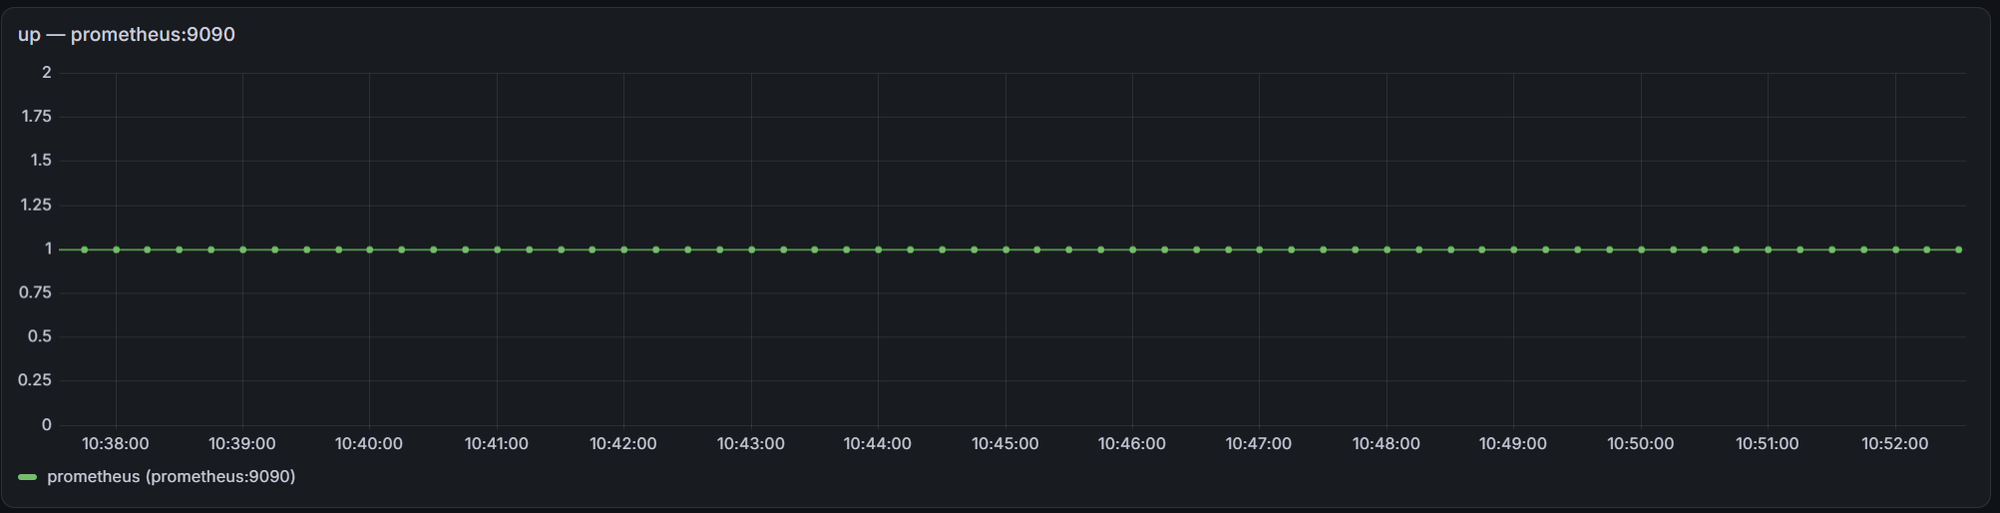
\includegraphics[width=\linewidth]{figures/grafana-prometheus-uptime.png}
  \caption{Dashboard \emph{Prometheus server uptime}: la métrica \code{up} de
  \code{prometheus:9090} se mantiene en 1.}
  \label{fig:uptime}
\end{figure}

%=====================================================================
\section{Práctica Observabilidad de Modelos}
%=====================================================================

\subsection{Métricas del modelo en la API}
Se añade \code{prometheus-client} a \code{requirements.txt} y en \code{app.py} un contador con
la etiqueta \code{species}, el endpoint \code{/metrics} y el incremento tras cada predicción.
La respuesta de \code{/predict} incluye ahora también la especie; la web solo lee
\code{prediction}, por lo que no cambia.

\begin{lstlisting}[language=python]
from prometheus_client import Counter, generate_latest, CONTENT_TYPE_LATEST

PREDICTION_COUNTER = Counter(
    'iris_prediction_count',
    'Contador de predicciones del modelo Iris por especie',
    ['species']
)

@app.route('/metrics')
def metrics():
    return Response(generate_latest(), mimetype=CONTENT_TYPE_LATEST)

# dentro de predict():
species_map = {0: 'setosa', 1: 'versicolor', 2: 'virginica'}
predicted_species = species_map.get(prediction_int, 'unknown')
PREDICTION_COUNTER.labels(species=predicted_species).inc()
return jsonify({'prediction': prediction_int, 'species': predicted_species})
\end{lstlisting}

\subsection{Verificación local}
Tras 30 predicciones de prueba (10 por especie), \code{curl localhost:5000/metrics} devuelve:

\begin{lstlisting}[style=plain]
iris_prediction_count_total{species="setosa"} 10.0
iris_prediction_count_total{species="versicolor"} 10.0
iris_prediction_count_total{species="virginica"} 10.0
\end{lstlisting}

El dashboard \emph{Predicciones IRIS} de Grafana representa
\code{iris\_prediction\_count\_total\{instance="mlops-api:5000"\}} con una serie por
especie. La figura~\ref{fig:iris-curl} muestra el estado tras esas 30 peticiones (las tres
series coinciden en 10 y se solapan); la figura~\ref{fig:iris-web}, la evolución al hacer
después predicciones desde la web de Streamlit (\code{http://localhost:8501}).

\begin{figure}[!htbp]
  \centering
  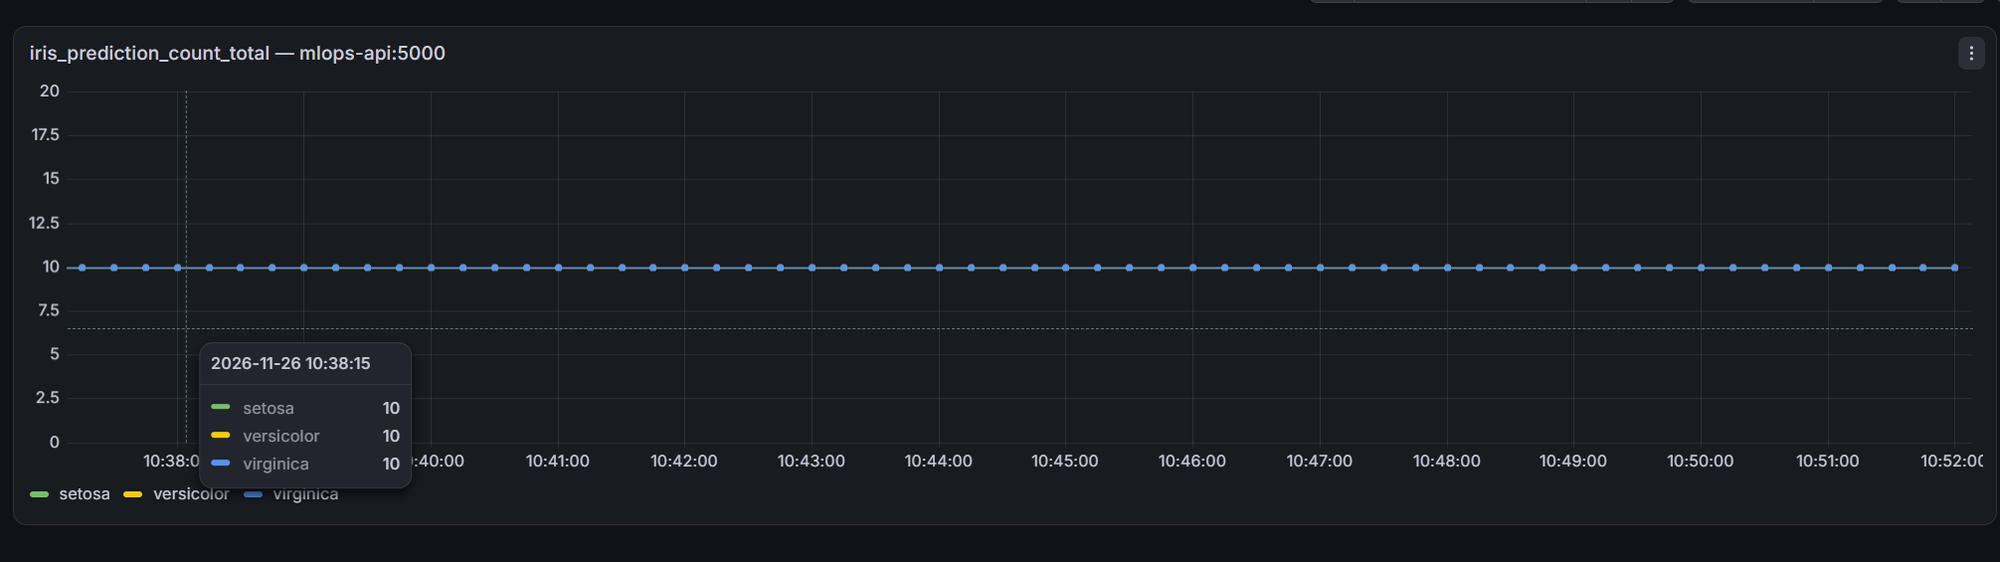
\includegraphics[width=\linewidth]{figures/grafana-predicciones-iris-curl.png}
  \caption{\emph{Predicciones IRIS} tras 30 peticiones a la API: 10 por especie.}
  \label{fig:iris-curl}
\end{figure}

\begin{figure}[!htbp]
  \centering
  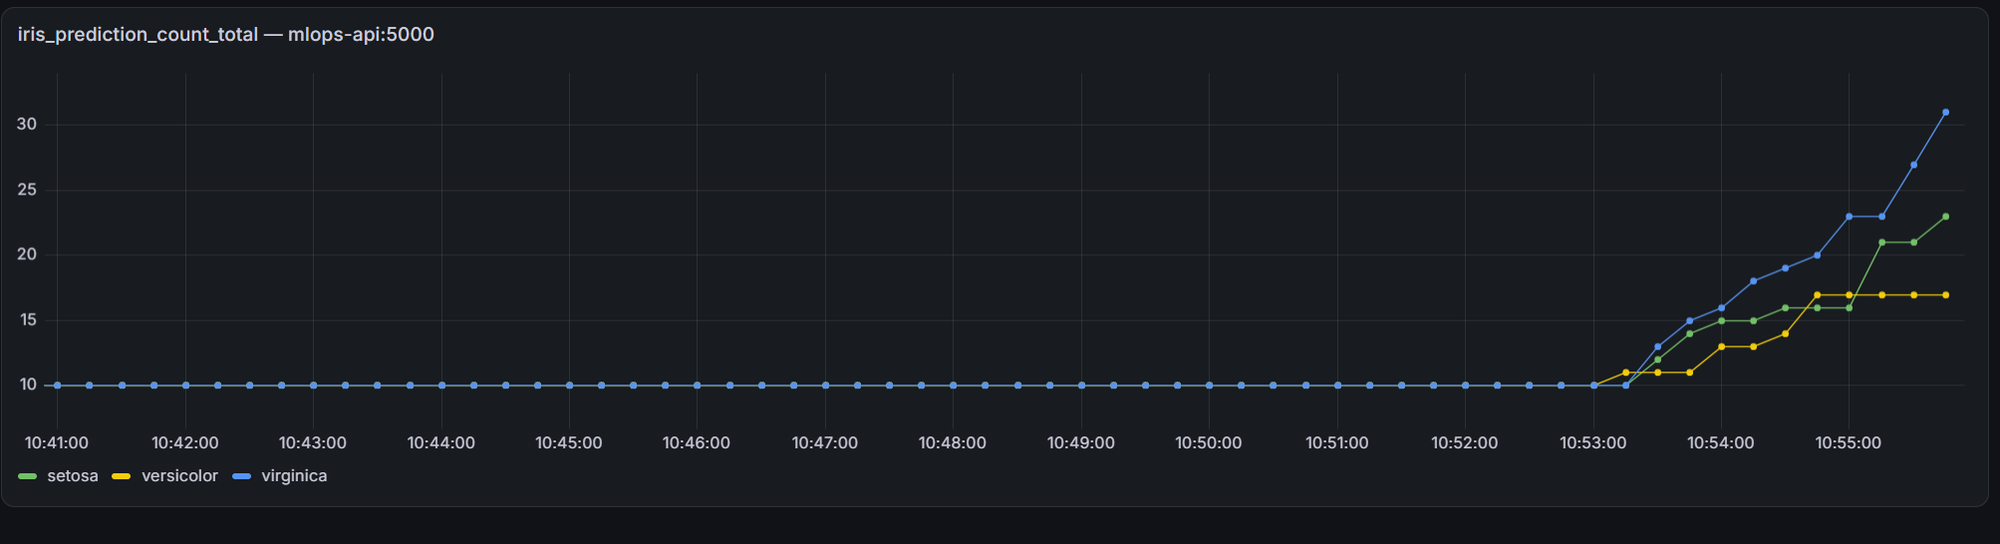
\includegraphics[width=\linewidth]{figures/grafana-predicciones-iris-web.png}
  \caption{\emph{Predicciones IRIS} con predicciones hechas desde la web a partir de las 10:53.}
  \label{fig:iris-web}
\end{figure}

\subsection{Manifiestos de Kubernetes}
GMP localiza el endpoint por el \emph{nombre} del puerto, así que el puerto 5000 pasa a
llamarse \code{metrics} en el Deployment y en el Service. En el Deployment se añadió además
una \code{readinessProbe} (ver sección~\ref{sec:dificultades}, dificultad~\ref{dif:readiness}).

\begin{lstlisting}[language=yaml]
# api-deployment.yaml (contenedor mlops-api)
        ports:
        - name: metrics
          containerPort: 5000
        readinessProbe:
          tcpSocket:
            port: metrics
          initialDelaySeconds: 2
          periodSeconds: 2
# api-service.yaml
  ports:
    - name: metrics
      protocol: TCP
      port: 5000
      targetPort: 5000
\end{lstlisting}

El recurso \code{PodMonitoring} (\code{pod-monitoring.yaml}) selecciona los pods
\code{app=mlops-api} y scrapea \code{/metrics} cada 30\,s:

\begin{lstlisting}[language=yaml]
apiVersion: monitoring.googleapis.com/v1
kind: PodMonitoring
metadata:
  name: mlops-api-pod-monitor
  namespace: default
spec:
  selector:
    matchLabels:
      app: mlops-api
  endpoints:
    - port: metrics
      path: /metrics
      interval: 30s
\end{lstlisting}

\subsection{Workflow de GitHub Actions}
El paso \emph{Deploy to GKE} aplica el \code{PodMonitoring} junto a los demás manifiestos, y
el \emph{smoke test} existente se amplió para comprobar que la predicción que acaba de hacer
aparece en las métricas y que el recurso existe:

\begin{lstlisting}[language=bash,style=plain]
kubectl apply -f api-deployment.yaml
kubectl apply -f api-service.yaml
kubectl apply -f pod-monitoring.yaml      # nuevo
...
kubectl exec deploy/mlops-web-deployment -- python -c "... requests.get(API_URL
  .replace('/predict', '/metrics')) ...; assert 'iris_prediction_count_total{species=' in m"
kubectl get podmonitoring mlops-api-pod-monitor
\end{lstlisting}

La ejecución \run{45792988289} termina en verde (\code{report/evidence/unit7-ci-ok-smoke.log}):

\begin{lstlisting}[style=plain]
deployment "mlops-api-deployment" successfully rolled out
deployment "mlops-web-deployment" successfully rolled out
iris_prediction_count_total***species="setosa"*** 2.0
mlops-api-pod-monitor   7m17s
Web: http://35.255.3.84
HTTP 200
WebSocket: HTTP/1.1 101 Switching Protocols
\end{lstlisting}

\begin{nota}[Los \code{***} del log]
GitHub enmascara en los logs cualquier fragmento que coincida con un secreto. La clave JSON
de \code{GCP\_SA\_KEY} contiene líneas \code{\{} y \code{\}}, así que las llaves de la línea
de la métrica aparecen como \code{***}. Es solo visual.
\end{nota}

El estado del \code{PodMonitoring} en el clúster es \code{ConfigurationCreateSuccess}
(\code{report/evidence/unit7-podmonitoring-status.yaml}).

\subsection{Métricas en Google Managed Prometheus}
Con más de 20 predicciones hechas desde la web desplegada en GKE, la métrica aparece en
\emph{Metrics Explorer} como \code{prometheus/iris\_prediction\_count\_total/counter} con una
serie por especie (figura~\ref{fig:gmp}). GMP añade las etiquetas
\code{cluster=mlops-gke-cluster}, \code{job=mlops-api-pod-monitor}, \code{namespace} y
\code{pod}. El tipo de recurso que muestra la consola es \emph{Prometheus Target}, no
\emph{Kubernetes Container} como indica el enunciado.

\begin{figure}[!htbp]
  \centering
  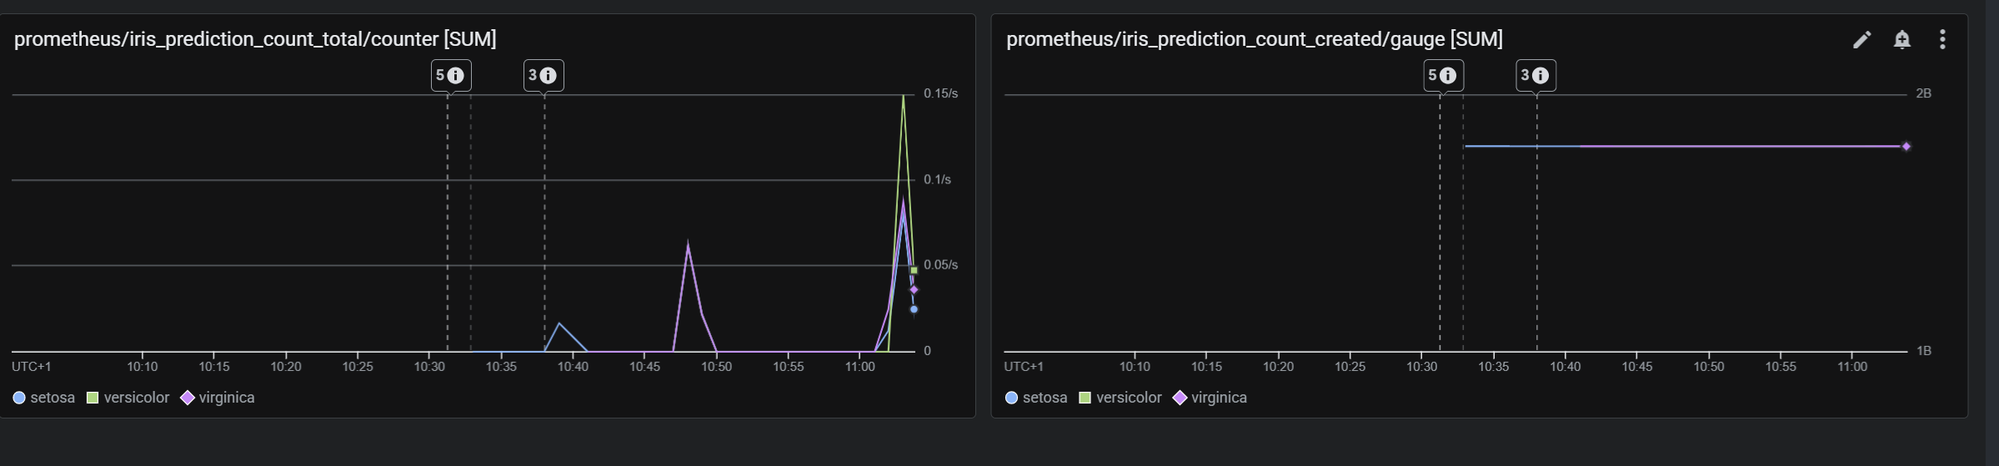
\includegraphics[width=\linewidth]{figures/gmp-metrics-explorer.png}
  \caption{Metrics Explorer: tasa de \metrica{} agrupada por especie (izquierda) y
  \code{iris\_prediction\_count\_created} (derecha, marca de tiempo de creación de cada serie).}
  \label{fig:gmp}
\end{figure}

La consulta PromQL del enunciado, \code{sum by (species) (iris\_prediction\_count\_total)},
lanzada contra la API PromQL de GMP (\code{report/evidence/unit7-gmp-promql.txt}) devuelve:

\begin{center}
\begin{tabular}{lr}
\toprule
\textbf{species} & \textbf{valor} \\
\midrule
setosa     & 19 \\
versicolor & 27 \\
virginica  & 25 \\
\bottomrule
\end{tabular}
\end{center}

\begin{pendiente}[Pendiente: captura de la consulta PromQL]
Falta la captura de Metrics Explorer con la consulta PromQL \emph{exacta}. La consola
convierte automáticamente la consulta del constructor en
\code{topk(30, sum by ("species")(rate(...)))}: hay que borrar todo el editor (también la
línea de comentario), pegar \code{sum by (species) (iris\_prediction\_count\_total)},
pulsar \emph{Run Query} y elegir \emph{Line chart}. Los datos siguen en Cloud Monitoring
aunque el clúster ya se haya borrado. Guardar como \code{figures/gmp-promql.png} y añadir
la figura aquí.
\end{pendiente}

\begin{nota}[Los totales de GMP empiezan en su primer scrape]
GMP toma la primera muestra que ve de un contador como punto de partida y solo cuenta los
incrementos posteriores. Las primeras 24 predicciones (que crearon las tres series entre dos
scrapes) quedaron como base y GMP mostró 0; tras 15 predicciones más (5 por especie) mostró
exactamente 5/5/5. Por eso los totales de Cloud Monitoring no coinciden con los que
devuelve \code{/metrics} en el pod, y por eso el enunciado pide alineación \emph{Delta}.
\end{nota}

%=====================================================================
\section{Registros de aplicación (Cloud Logging)}
%=====================================================================

\subsection{Logs de los pods}
\code{kubectl logs -l app=mlops-api} (desde Cloud Shell) muestra el scrape de GMP cada 30\,s,
igual que el ejemplo del enunciado (figura~\ref{fig:kubectl-logs}).

\begin{figure}[!htbp]
  \centering
  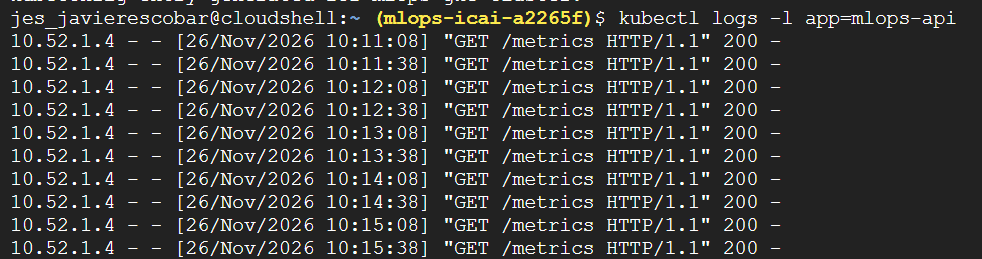
\includegraphics[width=0.85\linewidth]{figures/gke-kubectl-logs.png}
  \caption{\code{kubectl logs -l app=mlops-api}: el colector de GMP (\code{10.52.1.4})
  pide \code{/metrics} cada 30\,s.}
  \label{fig:kubectl-logs}
\end{figure}

\subsection{Filtros en el Explorador de registros}
Los dos filtros pedidos, sobre los contenedores de la API:

\begin{lstlisting}[style=plain]
resource.type="k8s_container"
labels."k8s-pod/app"="mlops-api"
severity="INFO"          # segundo filtro: severity>=INFO
\end{lstlisting}

\begin{figure}[!htbp]
  \centering
  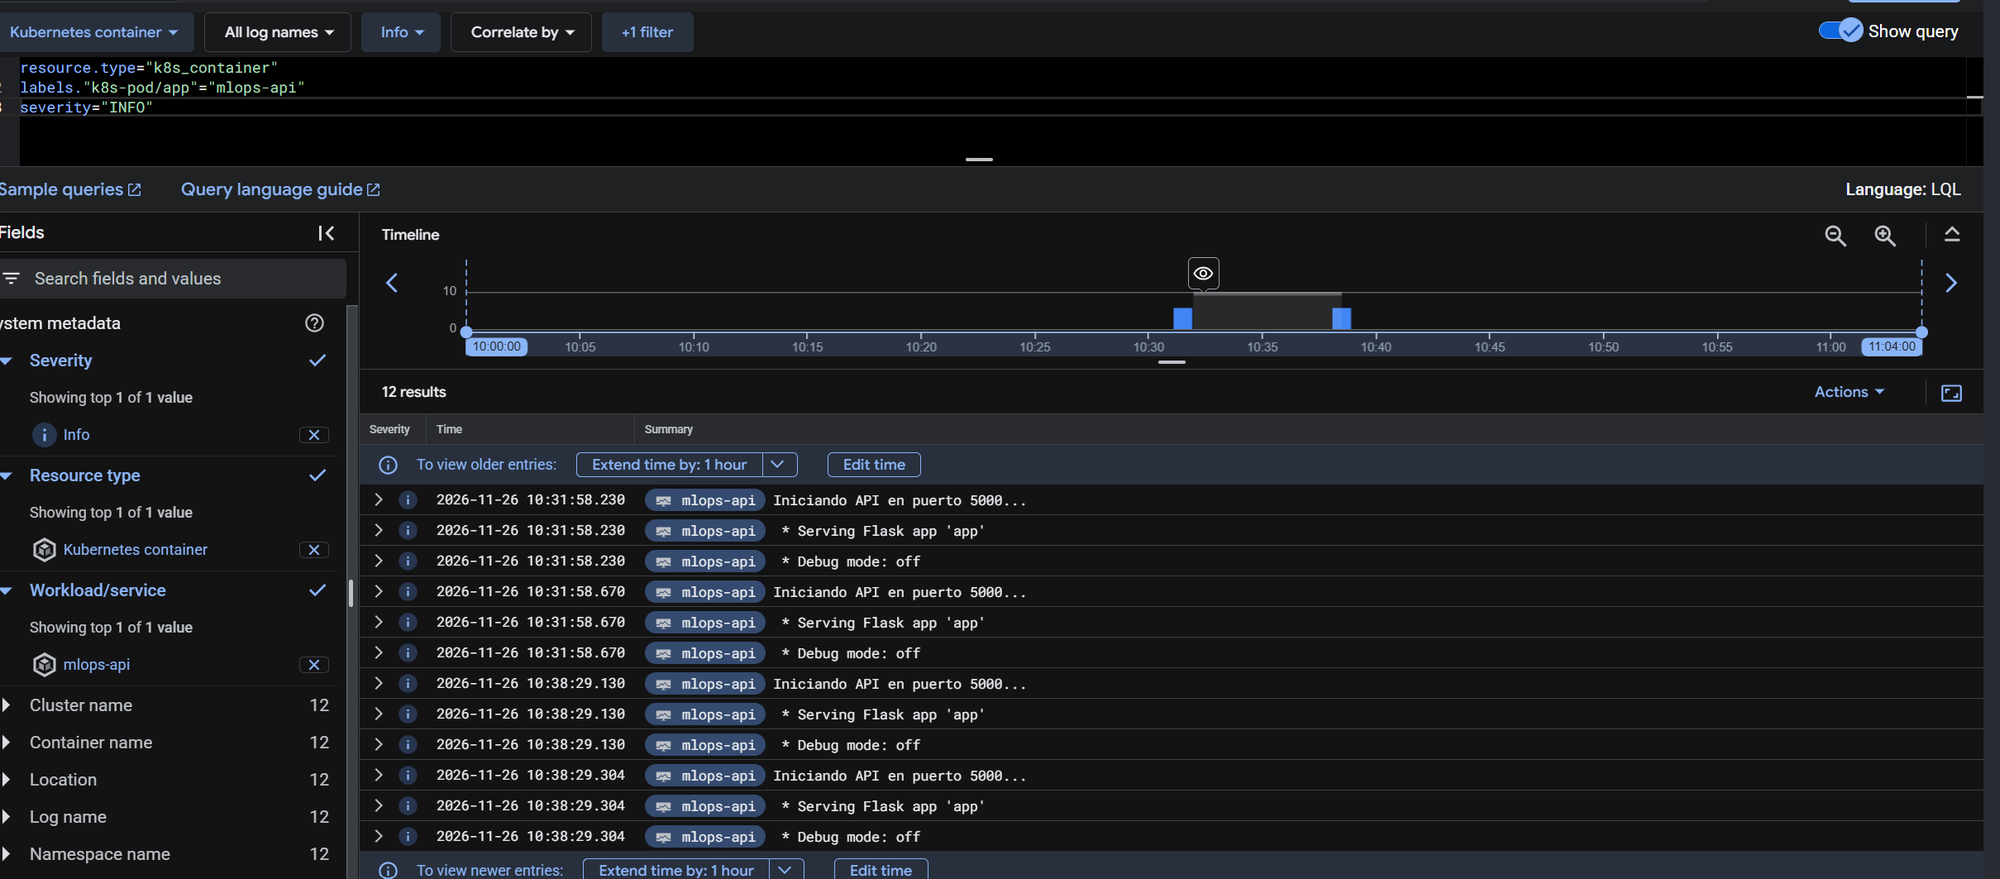
\includegraphics[width=\linewidth]{figures/logging-mlops-api-info.png}
  \caption{Filtro \code{severity="INFO"}: 12 resultados, solo los mensajes de arranque de
  Flask.}
  \label{fig:log-info}
\end{figure}

\begin{figure}[!htbp]
  \centering
  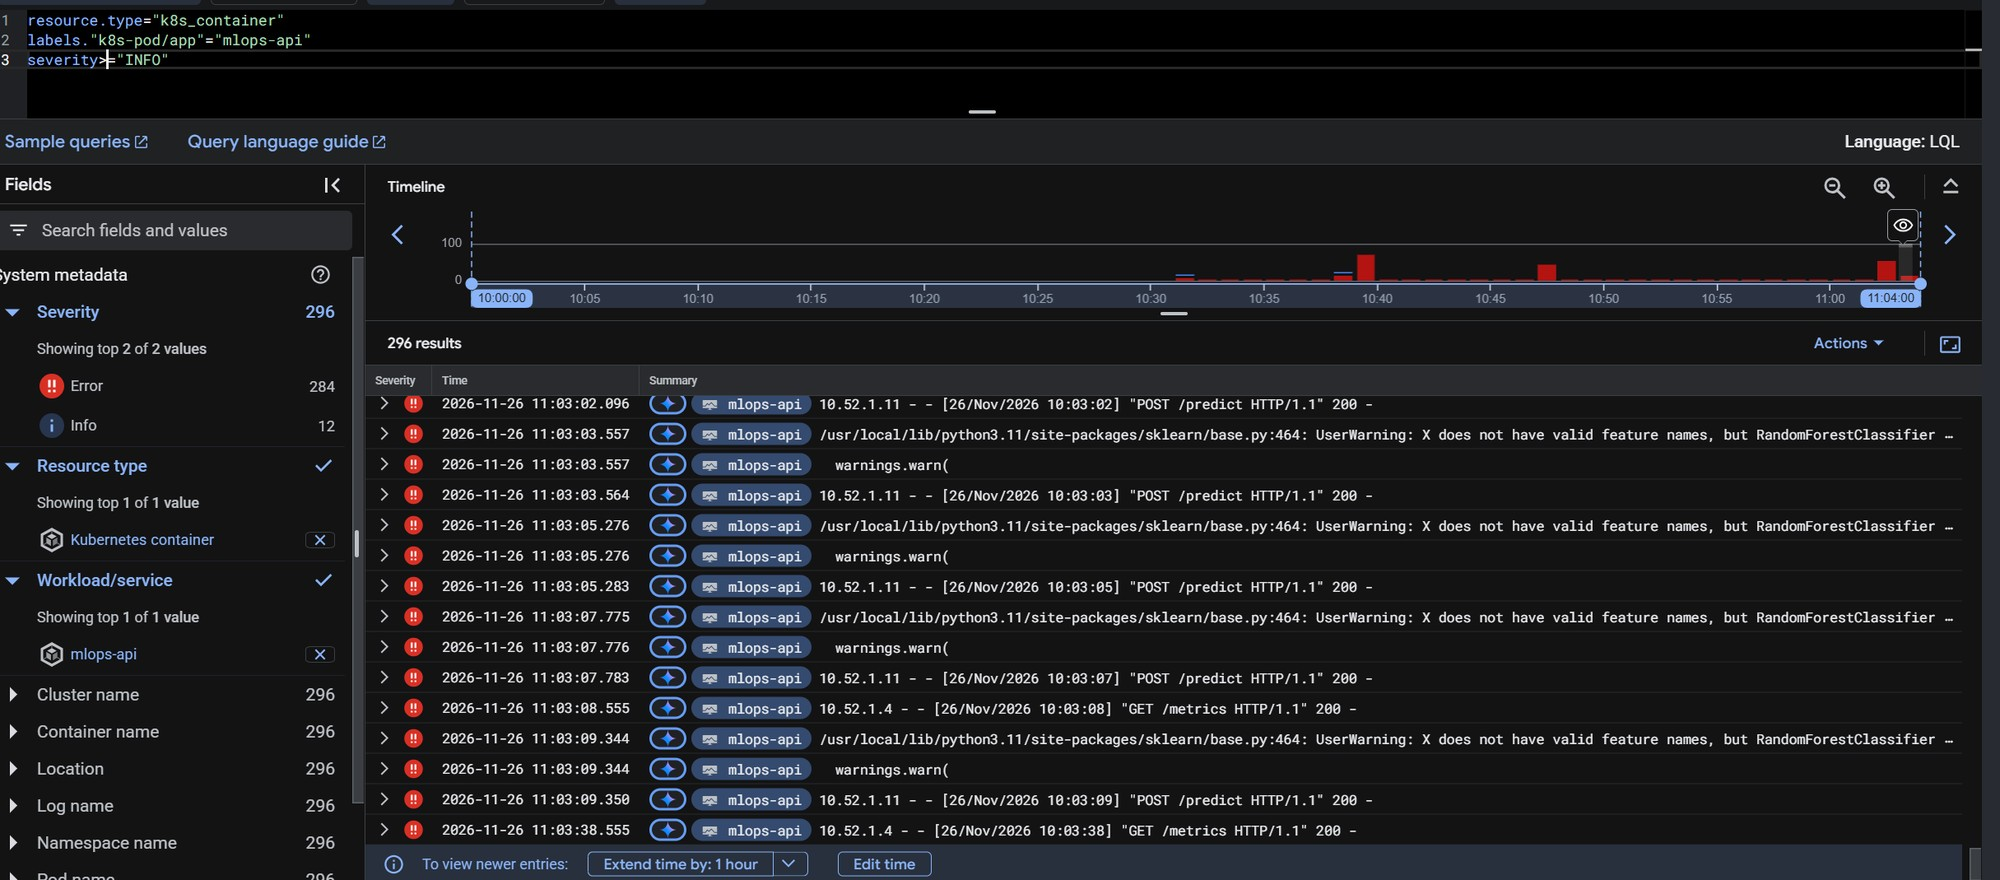
\includegraphics[width=\linewidth]{figures/logging-mlops-api-info-or-higher.jpg}
  \caption{Filtro \code{severity>=INFO}: 296 resultados (284 \emph{Error}, 12
  \emph{Info}). Las peticiones \code{POST /predict} y \code{GET /metrics} aparecen como
  \emph{Error}.}
  \label{fig:log-info-plus}
\end{figure}

\begin{aviso}[Las peticiones HTTP se registran como ERROR]
GKE asigna la severidad según el flujo de salida del contenedor: \code{stdout} se registra
como \code{INFO} y \code{stderr} como \code{ERROR}. El servidor de desarrollo de Flask
(werkzeug) escribe el log de cada petición en \code{stderr}, igual que el
\code{UserWarning} de scikit-learn (\emph{X does not have valid feature names}: el modelo se
entrenó con un DataFrame y la API le pasa un array de numpy). En las últimas 6\,h:
\code{severity="INFO"} devuelve 12 entradas y \code{severity>=INFO} 755 (743 \code{ERROR}),
\code{report/evidence/unit7-logging-severidad.txt}. Para que las peticiones salgan como
\code{INFO} bastaría con enviar el logging de Python a \code{stdout}
(\code{logging.basicConfig(stream=sys.stdout, level=logging.INFO)}) o usar logs JSON con un
campo \code{severity}; no se cambió para mantener el código del enunciado.
\end{aviso}

%=====================================================================
\section{Dashboard en Cloud Monitoring}
%=====================================================================
El enunciado pide dos gráficos con el total de predicciones por especie en la última hora,
uno \emph{Top List} y otro \emph{Gauge}, con alineación \emph{Delta}. El constructor actual
de la consola no ofrece ese alineador para esta métrica (solo la función de ventana tipo
\emph{rate}), así que el dashboard se definió como código y se creó con la API, donde
\code{ALIGN\_DELTA} sí existe:

\begin{lstlisting}[language=bash,style=plain]
gcloud monitoring dashboards create --project mlops-icai-a2265f \
  --config-from-file=cloud-monitoring/dashboard-predicciones-iris.json
\end{lstlisting}

\begin{itemize}[nosep]
  \item \textbf{Top List}: widget \code{timeSeriesTable} con \code{metricVisualization: BAR}.
  \item \textbf{Gauge}: widget \code{scorecard} con \code{gaugeView} (0--50). Un gauge solo
        representa una serie, así que hay uno por especie (filtrado por
        \code{metric.label.species}).
  \item En todos: métrica
        \code{prometheus.googleapis.com/iris\_prediction\_count\_total/counter},
        \code{perSeriesAligner: ALIGN\_DELTA}, \code{alignmentPeriod: 3600s},
        \code{crossSeriesReducer: REDUCE\_SUM}, \code{groupByFields: [metric.label.species]}.
\end{itemize}

\begin{lstlisting}[language=yaml,style=plain]
"aggregation": {
  "alignmentPeriod": "3600s",
  "perSeriesAligner": "ALIGN_DELTA",
  "crossSeriesReducer": "REDUCE_SUM",
  "groupByFields": ["metric.label.\"species\""]
}
\end{lstlisting}

Para la hora 10:20--11:20 (CET), que incluye las predicciones hechas desde la web, el
dashboard muestra setosa 12, versicolor 15 y virginica 13 (figura~\ref{fig:dashboard}); la
misma agregación lanzada contra la API \code{timeSeries.list} devuelve los mismos valores.

\begin{figure}[!htbp]
  \centering
  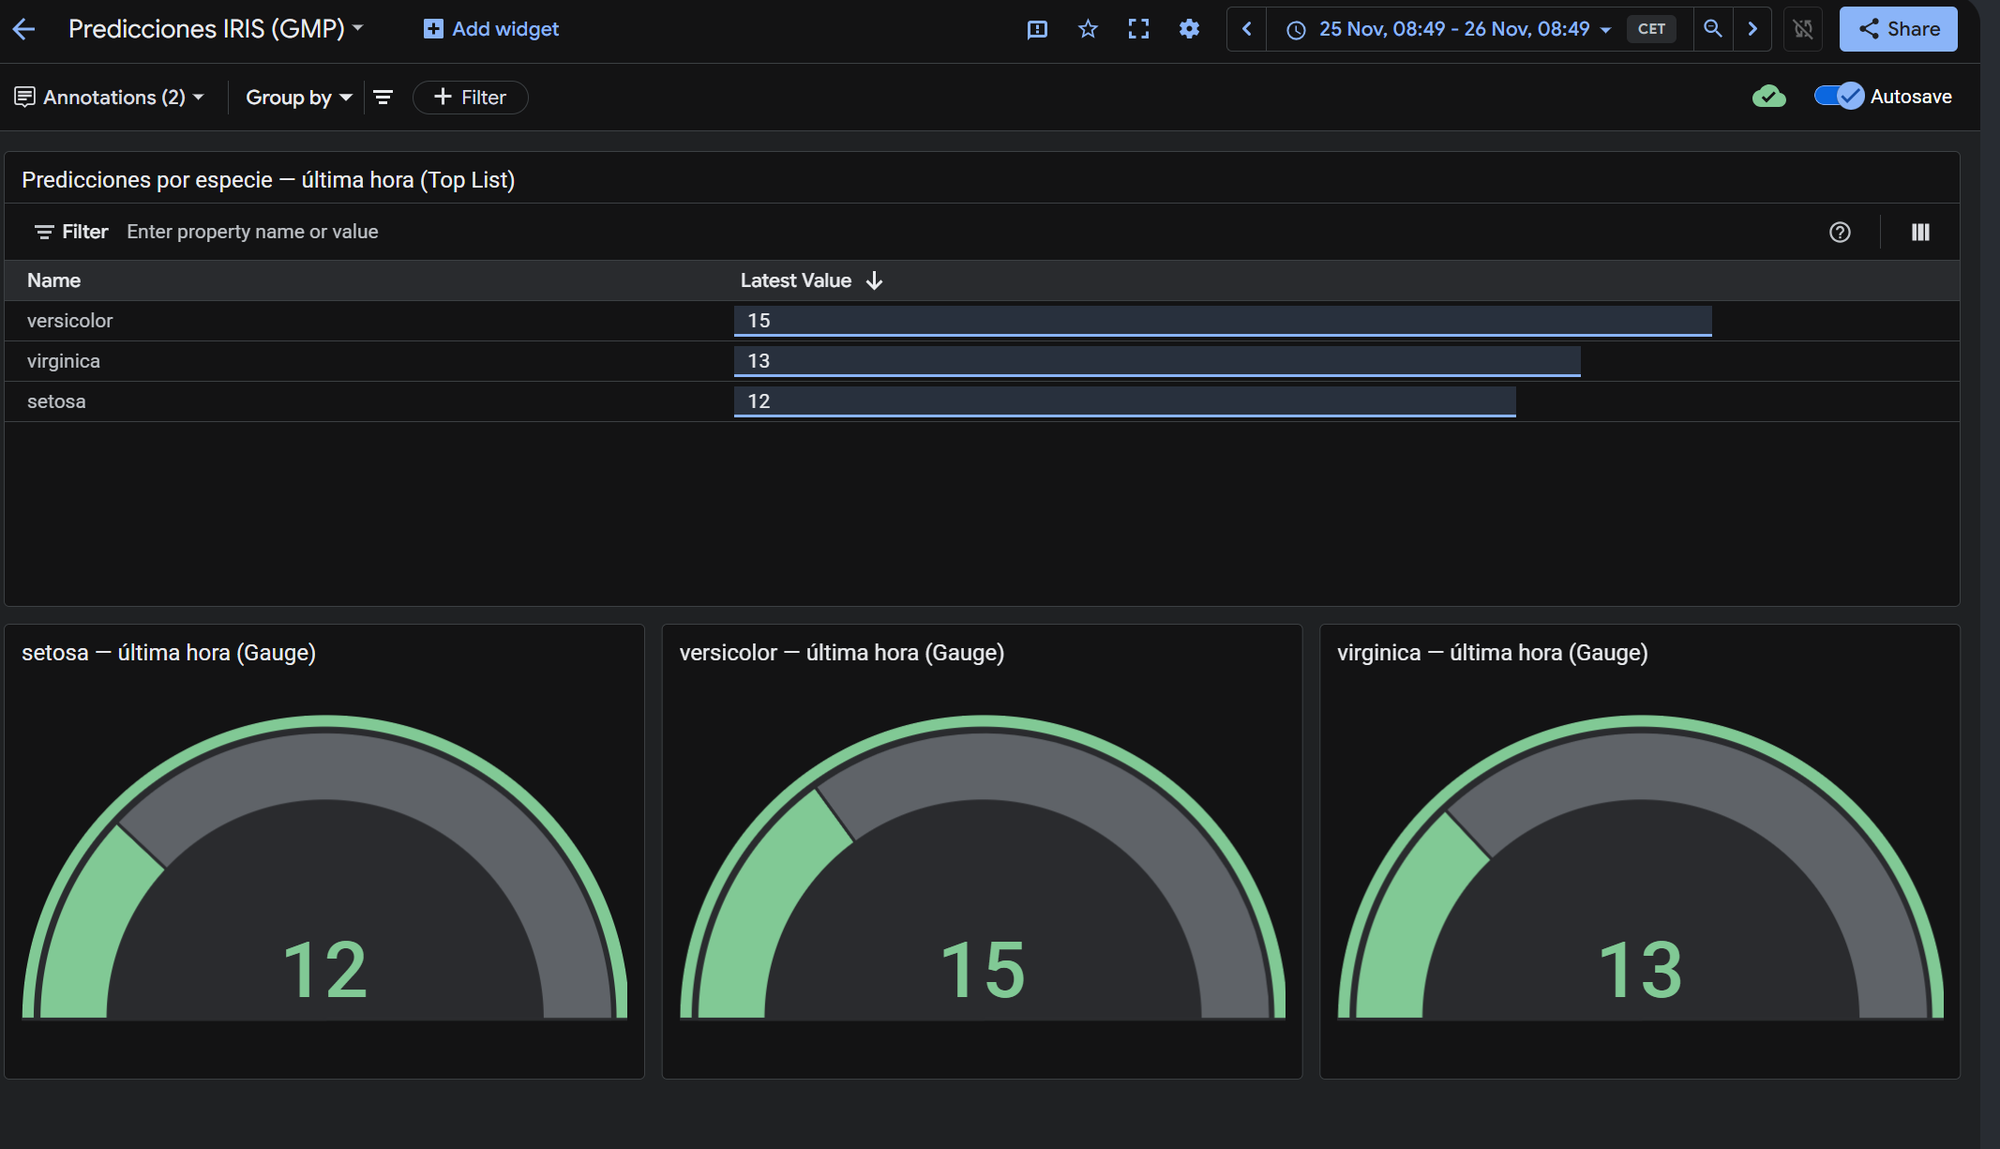
\includegraphics[width=\linewidth]{figures/cloud-monitoring-dashboard.png}
  \caption{Dashboard \emph{Predicciones IRIS (GMP)}: Top List y un Gauge por especie,
  alineación Delta de 1\,h.}
  \label{fig:dashboard}
\end{figure}

%=====================================================================
\section{Dificultades y soluciones}\label{sec:dificultades}
%=====================================================================

\begin{enumerate}[label=\textbf{D\arabic*.}, ref=D\arabic*, leftmargin=2.4em, itemsep=0.5em]

\item \textbf{El clúster ya no existía.} Se había borrado al acabar la Unit 4.
  \emph{Solución:} recrearlo con el mismo nombre (las variables de GitHub Actions apuntan a
  él) y con \code{--enable-managed-prometheus --logging=SYSTEM,WORKLOAD}, lo que hace
  innecesarios los dos \code{clusters update} del enunciado.

\item \textbf{\code{kubectl} local sin acceso al clúster}
  (\code{gke-gcloud-auth-plugin not found}). El SDK de gcloud no tenía el plugin.
  \emph{Solución:} \code{gcloud components install gke-gcloud-auth-plugin}.

\item \textbf{Docker Compose usaba la imagen de Docker Hub.} El \code{docker-compose.yml}
  apuntaba a \code{jes0406/mlops-api}, que no tiene \code{/metrics}; el \code{docker build}
  del enunciado genera \code{mlops-api:latest}, que Compose nunca usaba.
  \emph{Solución:} \code{build: .} en el servicio de la API.

\item \textbf{El \code{.gitignore} ignoraba todos los \code{*.json}} (pensado para métricas
  de MLflow), incluidos los dashboards. \emph{Solución:} excepciones
  \code{!grafana-provisioning/dashboards/*.json} y \code{!cloud-monitoring/*.json}.

\item \textbf{Grafana con contraseña por defecto expuesta en la red.} El enunciado fija
  \code{admin}/\code{admin}; publicar el puerto en todas las interfaces lo deja accesible
  desde la LAN. \emph{Solución:} publicar Grafana y Prometheus solo en \code{127.0.0.1}.
  \code{http://localhost:3000} sigue funcionando igual.

\item \label{dif:readiness}\textbf{Primer despliegue en rojo: \emph{Connection refused}}
  (\run{45791953319}, \code{report/evidence/unit7-ci-fallo-readiness.log}).
  \code{kubectl rollout status} dio el despliegue por terminado a las 09:31:53, el smoke test
  llamó a la API a las 09:31:56 y Flask no empezó a escuchar hasta las 09:31:58: sin
  \emph{readiness probe}, Kubernetes marca el pod como listo en cuanto arranca el contenedor,
  antes de que Python cargue scikit-learn y el modelo. En un clúster nuevo, con las imágenes
  sin cachear, el margen era aún menor. \emph{Solución:} \code{readinessProbe} TCP sobre el
  puerto \code{metrics} (TCP y no HTTP para no añadir más peticiones a \code{/metrics} en los
  logs). La siguiente ejecución, \run{45792988289}, pasó.

\item \textbf{La web pública de GKE no cargaba desde la red de casa.}
  \code{http://35.255.3.84} respondía \code{HTTP 200}, pero la página de Streamlit se
  quedaba sin cargar. Streamlit necesita un WebSocket (\code{/\_stcore/stream}); desde
  nuestra red la petición de \emph{upgrade} recibía \emph{Connection reset by peer} siempre,
  mientras que desde el runner de GitHub (CI) y a través de \code{kubectl port-forward}
  devolvía \code{101 Switching Protocols}. El servidor estaba bien: algo en la red local
  (antivirus, proxy o el router/ISP) corta los WebSockets en el puerto 80.
  \emph{Solución:} hacer las predicciones a través de
  \code{kubectl port-forward svc/mlops-web-service 8080:80} y \code{http://localhost:8080}.
  Las peticiones siguen pasando por la web y la API desplegadas en GKE, así que cuentan en GMP.

\item \textbf{El \code{port-forward} se caía} (\emph{lost connection to pod}) cuando un
  cliente cerraba una conexión de golpe. \emph{Solución:} relanzarlo en un bucle
  \code{while true; do kubectl port-forward ...; done}.

\item \textbf{\code{kubectl} en Cloud Shell intentaba conectar a \code{localhost:8080}.}
  Cloud Shell no tenía credenciales del clúster. \emph{Solución:}
  \code{gcloud container clusters get-credentials mlops-gke-cluster --zone us-central1-a}.

\item \textbf{Totales de GMP distintos a los del pod.} GMP usa la primera muestra de cada
  serie como base (ver la nota de la sección de GMP). \emph{Solución:} interpretarlo con
  \emph{Delta}/\code{increase} y verificarlo: 15 predicciones adicionales se reflejaron
  exactamente.

\item \textbf{Métrica equivocada en Metrics Explorer.} El primer gráfico salía en miles de
  millones: era \code{iris\_prediction\_count\_created}, que guarda la marca de tiempo Unix
  de creación de cada serie (y, sumada sobre tres especies, $\approx 5{,}4\cdot 10^9$).
  \emph{Solución:} usar \metrica{} y agrupar por \code{species}.

\item \textbf{Filtros de logs sin la etiqueta de la app.} Sin
  \code{labels."k8s-pod/app"="mlops-api"} el explorador mezcla logs de todo el clúster
  (konnectivity-agent, auditoría del API server\ldots). \emph{Solución:} usar el editor de
  consultas con las tres condiciones.

\item \textbf{Peticiones HTTP con severidad ERROR}: ver el aviso de la sección de logs.
  Se documenta en vez de cambiar el código.

\item \textbf{Sin alineador Delta en la consola de Cloud Monitoring.}
  \emph{Solución:} dashboard como código (JSON) creado con
  \code{gcloud monitoring dashboards create}; un Gauge por especie porque el widget solo
  representa una serie.

\item \textbf{Ejecución de CI innecesaria.} El commit del JSON del dashboard no llevaba
  \code{[skip ci]} y disparó entrenamiento y despliegue (\run{45824018641}).
  \emph{Solución:} cancelarla; los commits que solo añaden capturas llevan \code{[skip ci]}.

\end{enumerate}

%=====================================================================
\section{Limpieza}
%=====================================================================
\begin{itemize}[nosep]
  \item Antes de borrar el clúster se eliminó el Service \code{LoadBalancer} de la web, para
        que GKE libere la regla de reenvío y la IP pública (si se borra solo el clúster
        pueden quedar huérfanas y seguir facturando). Después:
        \code{gcloud container clusters delete mlops-gke-cluster --zone us-central1-a}.
  \item Las evidencias del clúster (recursos, estado del \code{PodMonitoring}, PromQL, logs)
        se guardaron antes en \code{report/evidence/unit7-*}.
  \item Se mantienen el dashboard de Cloud Monitoring y las métricas de GMP, que no tienen
        coste por existir y siguen consultables.
\end{itemize}

%=====================================================================
\section*{Ficheros entregados}
%=====================================================================
\small
\begin{tabularx}{\linewidth}{@{}>{\raggedright\arraybackslash}p{0.47\linewidth}>{\raggedright\arraybackslash}X@{}}
\toprule
\textbf{Fichero} & \textbf{Contenido} \\
\midrule
\code{docker-compose.yml} & API construida en local, Prometheus y Grafana (en localhost) \\
\code{prometheus.yaml} & Scrape de \code{prometheus:9090} y \code{mlops-api:5000} \\
\code{grafana-provisioning/} & Datasource y dashboards \emph{Prometheus server uptime} y \emph{Predicciones IRIS} \\
\code{app.py}, \code{requirements.txt} & Contador \metrica{} y endpoint \code{/metrics} \\
\code{api-deployment.yaml}, \code{api-service.yaml} & Puerto \code{metrics} y \emph{readiness probe} \\
\code{pod-monitoring.yaml} & \code{PodMonitoring} para GMP \\
\code{.github/workflows/cml.yaml} & Aplica el \code{PodMonitoring} y comprueba \code{/metrics} \\
\code{cloud-monitoring/}\allowbreak\code{dashboard-predicciones-iris.json} & Dashboard Top List + Gauges (Delta) \\
\code{report/evidence/unit7-*} & Evidencias de CLI, CI, GMP y Cloud Logging \\
\bottomrule
\end{tabularx}

\end{document}
